\section{Two-sample testing for networks}
\paragraph*{Co-authored with Sambit Panda}
\label{sec:ch8:twosample}

In Section \ref{sec:ch6:multinet}, we learned several techniques for dealing with multiple networks. When you find networks in your data, a fundamental question that you might have is how to determine whether the networks differ. This problem is another instance of a two-sample test, much like the two-sample test that we learned about in Section \ref{sec:ch7:testing:twosample}. Remember that a \textit{two-sample test} was a test to determine whether two samples of data were different. 

To do this, we'll return to the alien and human brain networks example, from Case Study \ref{box:ch6:multinet:ex}. There are $n=100$ brain areas, which represent the nodes of the network. This time, we find a third group of aliens, and their brain structure is much more similar to humans than our original group of aliens (they are still homophilic). However, this group of aliens tends to have heterogeneities in the node degrees: nodes with lower indices have a higher degree than nodes with higher indices, whereas the human brains tend to have more homogeneous structurings.

Let's imagine that we have one human brain, and one alien brain:

\begin{lstlisting}[style=python]
from graspologic.simulations import sbm
import numpy as np
from graphbook_code import dcsbm, generate_dcsbm_pmtx, \
                           generate_sbm_pmtx

n = 100  # the number of nodes
M = 8  # the total number of networks
# human brains have homophilic block structure
Bhum = np.array([[0.2, 0.02], [0.02, 0.2]])
# alien brains add degree-correction
theta_alien = np.tile(np.linspace(1.7, 0.3, 50), 2)

# generate 4 human and alien brain networks
A_human, z = sbm([n // 2, n // 2], Bhum, return_labels=True)
A_alien = dcsbm(z, theta_alien, Bhum)

Phum = generate_sbm_pmtx(z, Bhum)
Palien = generate_dcsbm_pmtx(z, theta_alien, Bhum)
\end{lstlisting}

Plots of the networks are shown in Figure \ref{fig:ch8:twosample:ex}, where their underlying probability matrices are shown in \textbf{(A)} and \textbf{(C)}. Note that the degree-correction factor for the alien brain network has led to the nodes with lower indices in each community to have higher probabilities of being connected to other nodes. Samples of the human and alien brain networks are \textbf{(B)} and the alien brain network in \textbf{(D)}. It is a little bit less obvious that the networks are different when we look at the network samples. 

Just like when we were flipping coins we could not immediately conclude that two coins were different just because they produced a different number of heads in a given number of flips, it would be unwise to conclude that the networks differ fundamentally (they have different probability matrices) just because the samples look different. 

\begin{figure}[h]
    \centering
    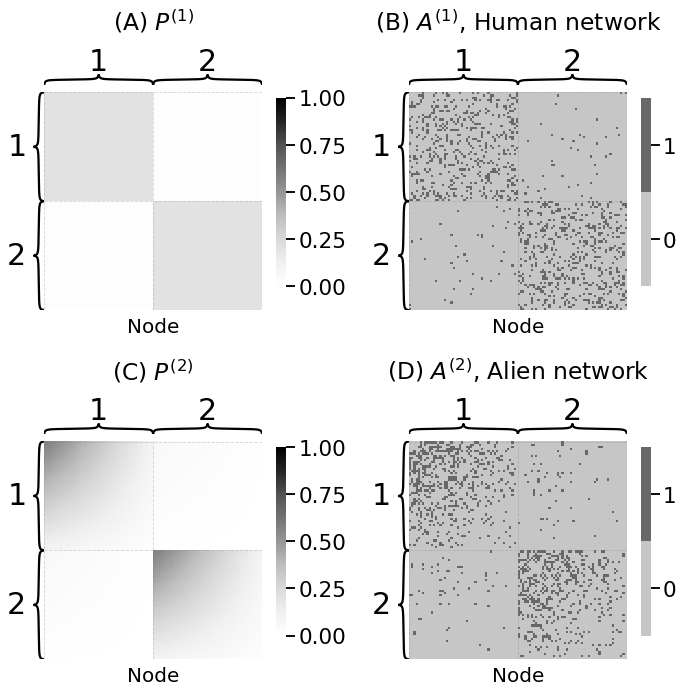
\includegraphics[width=0.7\linewidth]{applications/ch8/Images/ts_ex.png}
    \caption[Human and alien brains]{\textbf{(A)} probability matrix underlying human brain network, \textbf{(B)} brain network from human, \textbf{(C)} probability matrix underlying alien brain network, \textbf{(D)} brain network from alien.}
    \label{fig:ch8:twosample:ex}
\end{figure}

For this reason, it is important for us to build out our two-sample testing procedures, so that we can determine whether the networks differ.

\subsection{Two-sample tests and random networks}

In this section, we'll go a slightly different direction from the last time we saw two-sample testing. When we have two random networks $\mathbf A^{(1)}$ and $\mathbf A^{(2)}$, our first thing that we need to do is determine appropriate models for our networks. If we make the assumption that these networks are $IER_n\left(P^{(m)}\right)$ random networks from Section \ref{sec:ch5:ier}, which are the broadest class of independent-edge random network models, remember that the probability matrix encodes the differences between the two random networks. Therefore, our question is:
\begin{align*}
    H_0 : P^{(1)} = P^{(2)} \text{ against }H_A : P^{(1)} \neq P^{(2)}, \numberthis \label{eqn:ch8:twosample:2shypo_prob}
\end{align*}
or that the edge probability matrices are the same (under the null hypothesis) against that the edge probability matrices differ (under the alternative hypothesis). This is exactly the same question that we would ask about determining whether two coins are different, but generalized to $n \times n$ probability matrices.

Remember, however, that the $IER_n\left(P^{(m)}\right)$ random networks are difficult to deal with (directly) when you only have a single network sample. This means that testing the hypotheses in Equation \eqref{eqn:ch8:twosample:2shypo_prob} is fairly impractical when you only have two networks, because you only have one sample $a_{ij}^{(m)}$ to base your estimate of $p_{ij}^{(m)}$ on. 

\subsection{Latent positition testing}
\label{sec:ch8:twosample:lpt}
For this reason, it is fairly typical to make further assumptions about the network structure. As you learned in Section \ref{sec:ch6:ase}, a typical assumption that we can make is that the networks are $RDPG_n\left(X^{(m)}\right)$ random networks, with latent position matrices $X^{(m)}$. Remember that your latent position matrix $X^{(m)}$ fully describes the probability matrix $P^{(m)}$, so it would be (almost) equivalent to just compare the latent positions directly:
\begin{align*}
    H_0 : X^{(1)} = X^{(2)} \text{ against }H_A : X^{(1)} \neq X^{(2)}, \numberthis \label{eqn:ch8:twosample:2shypo_lpm:dumb}
\end{align*}
or would it? Remember that for a network with a latent position matrix $X^{(m)}$, that for any $d \times d$ rotation matrix $W$, by the non-identifiability problem in Section \ref{sec:ch6:spectral:nonidentifiable}:
\begin{align*}
    P^{(m)} &= X^{(m)}X^{(m)}^\top = X^{(m)}WW^\top X^{(m)}^\top
\end{align*}
This means that even if $P^{(1)}$ and $P^{(2)}$ were identical, we could define their latent position matrices differently, and still end up with the same random network, by having $X^{(2)} = X^{(1)}W$ for some rotation matrix $W$. For this reason, we'll make our hypothesis ``robust'' to this challenge, and test:
\begin{align*}
    H_0 :& X^{(1)} = WX^{(2)}\text{ for some rotation matrix $W$} \\
    H_A :& X^{(1)} \neq WX^{(2)} \text{ for any rotation matrix $W$}. \numberthis \label{eqn:ch8:twosample:2shypo_lpm:smart}
\end{align*}
In words, our null hypothesis is that the latent positions are identical up to a rotation (for some possible rotation matrix), and our alternative hypothesis is that the latent positions are not rotations of one another (for any possible rotation matrix). 

\subsubsection*{Learning rotations from the data}

From Section \ref{sec:ch6:ase}, we know that we can obtain estimates of $X^{(m)}$ by using the \texttt{ase}, where $\hat X^{(m)} = \texttt{ase}\left(A^{(m)}\right)$. How do we account for the potential that $X^{(1)}$ and $X^{(2)}$ are rotations of one another?

\paragraph*{The orthogonal Procrustes problem}

To estimate a possible rotation, we will need to set up an optimization problem. Our goal is to find the best possible rotation of $X^{(2)}$ onto $X^{(1)}$. 

\begin{floatingbox}[h]\caption{Concept: The Frobenius norm}
\label{box:ch7:twosample:frobnorm}
The Frobenius norm can be thought of as a generalization of the Euclidean norm from Concept \ref{def:ch6:se:eucl_dist} to matrices. If $A$ is a $n \times m$ matrix with entries $a_{ij}$, the Frobenius norm is:
\begin{align*}
    \|A\|_F &= \sqrt{\sum_{i = 1}^n \sum_{j = 1}^m a_{ij}}
\end{align*}
We can use the Frobenius norm to define a distance. If $A$ and $B$ are two matrices with the same number of rows ($n$) and columns ($m$), their Frobenius distance is:
\begin{align*}
    \|A - B\|_F &= \sqrt{\sum_{i = 1}^n \sum_{j = 1}^m (a_{ij} - b_{ij})^2}
\end{align*}
\end{floatingbox}

Using Concept \ref{box:ch7:twosample:frobnorm}, we can define what we mean by the ``best'' possible rotation: the rotation where the Frobenius distance between $X^{(1)}$ and $X^{(2)}$ are minimized. We can describe our goal as:
\begin{align*}
    \text{find }W \text{ where } \left\|X^{(1)} - X^{(2)}W\right\|_F\text{ is minimized}.
\end{align*}
We can equivalently write this goal as:
\begin{align*}
    \hat W &= \text{argmin}_W \left\|X^{(1)} - X^{(2)}W\right\|_F.\numberthis \label{eqn:ch8:twosample:opp}
\end{align*}
The idea is that if $X^{(1)}$ and $X^{(2)}$ are rotations of one another, we can (at least, in theory) for the $d \times d$ rotation matrix $\hat W$ that properly aligns them. If such a rotation exists, the function that we are minimizing $\left\|X^{(1)} - X^{(2)}\hat W\right\|_F$ will have a value of $0$ when we find the correct rotation (because the matrices will be identical). The problem of solving for optimal rotations in Equation \eqref{eqn:ch8:twosample:opp} is known as the \textit{orthogonal Procrustes problem}.

In practice, we only have estimates $\hat X^{(1)}$ and $\hat X^{(2)}$, so we will not find the perfect rotation of $\hat X^{(1)}$ onto $\hat X^{(2)}$ (even if such a rotation exists for $X^{(1)}$ and $X^{(2)}$). Therefore, when we minimize $\left\|\hat X^{(1)} - \hat X^{(2)}W\right\|_F$, we will just want the $\hat W$ that makes them the most similar (in terms of the Frobenius distance). If $X^{(1)}$ and $X^{(2)}$ are the same, we would expect that $\left\|\hat X^{(1)} - \hat X^{(2)}\hat W\right\|_F$ would therefore take a relatively small value.

Programatically, we can code this up as:

\begin{lstlisting}[style=python]
from scipy.linalg import orthogonal_procrustes
from graspologic.models import RDPGEstimator
import numpy as np

d = 2
# estimate latent positions for alien and human networks
Xhat_human = RDPGEstimator(n_components=d).fit(A_human).latent_
Xhat_alien = RDPGEstimator(n_components=d).fit(A_alien).latent_
# estimate best possible rotation of Xhat_alien to Xhat_human by 
# solving orthogonal procrustes problem
W = orthogonal_procrustes(Xhat_alien, Xhat_human)[0]
observed_norm = np.linalg.norm(Xhat_human - Xhat_alien @ W, ord="fro")
\end{lstlisting}

This gives us the value shown in Figure \ref{fig:ch8:twosample:lpt}(A), in gray. A relatively small value, relative what exactly?

\begin{figure}
    \centering
    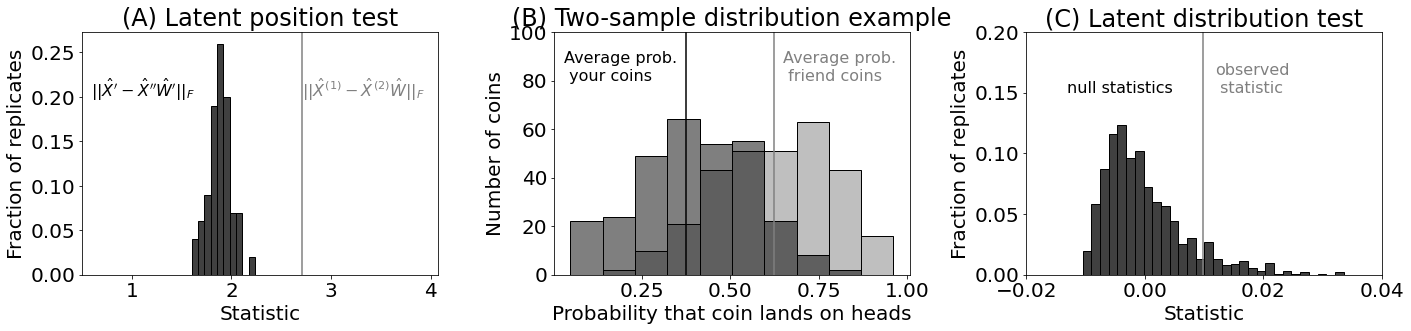
\includegraphics[width=\linewidth]{applications/ch8/Images/ts_ldt_ex.png}
    \caption[Latent position and latent distribution testing]{\textbf{(A)} The observed statistic from the data (gray) compared to a histogram from the $r=100$ parametric replicates (black). \textbf{(B)} A comparison of two buckets of coins, where each coin has a different probability of landing on heads. \textbf{(C)} The observed statistic from the data (gray) compared to a histogram from the $r=1000$ replicates (black).}
    \label{fig:ch8:twosample:lpt}
\end{figure}

\subsubsection{Generating a null distribution through parametric bootstrapping}

If you recall from Section \ref{sec:ch7:testing:twosample}, we learn with hypothesis tests by looking at how well the data reflect the null hypothesis; that is, that the estimated latent positions (computed from the data) are identical (up to a rotation). 

When you have estimates computed from the data, ideally, you will be able to determine directly (by the nature of the data and the assumptions that you make) exactly how ``anomalous'' the difference that you observe is relative what you would expect under the null hypothesis. In the case of the contingency tables from Section \ref{sec:ch7:testing:twosample}, the Fisher's exact test used the assumptions that we made (that the two samples were independent binary events) to compute how ``anomalous'' the contingency table that we observed was. 

In this case, however, without more assumptions we can't quite compute this value exactly. In the interest of keeping assumptions to a minimum, a popular strategy is to use what is known as a \textit{bootstrap}. A \textit{bootstrap} is a technique which attempts to quantify the sampling distribution of some quantity (a \textit{statistic}) that is computed from the data. The \textit{sampling distribution} refers to the distribution of the statistic $\left\|\hat X^{(1)} - \hat X^{(2)}\hat W\right\|_F$, where $\hat X^{(1)}$, $\hat X^{(2)}$, and $\hat W$ are computed from the data.

The way that we will do this is that we will use the parameter $\hat X^{(1)}$ as the latent position matrix for two new random networks, $\mathbf A'$ and $\mathbf A''$. These two random networks have an identical latent position matrix: $\hat X^{(1)}$. Then, we will generate two new samples of these random networks with the same latent position matrix:

\begin{lstlisting}[style=python]
from graspologic.simulations import rdpg

def generate_synthetic_networks(X):
    """
    A function which generates two synthetic networks with
    same latent position matrix X.
    """
    A1 = rdpg(X, directed=False, loops=False)
    A2 = rdpg(X, directed=False, loops=False)
    return A1, A2

Ap, App = generate_synthetic_networks(Xhat_human)
\end{lstlisting}

We then use these two new networks, and again estimate latent position matrices for these:

\begin{lstlisting}[style=python]
def compute_latent(A, d):
    """
    A function which returns the latent position estimate
    for an adjacency matrix A.
    """
    return RDPGEstimator(n_components=d).fit(A).latent_

Xhat_p = compute_latent(Ap, d)
Xhat_pp = compute_latent(App, d)
\end{lstlisting}

Finally, just like we aligned $\hat X^{(1)}$ and $\hat X^{(2)}$ via the ``optimal rotation'' $\hat W$, we will align $\hat X'$ and $\hat X''$ via the ``optimal rotation'' $\hat W'$. Then, we recompute our statistic of interest $\left\|\hat X' - \hat X''W'\right\|_F$ using these new samples, where the underlying latent positions were truly identical:

\begin{lstlisting}[style=python]
def compute_norm_orth_proc(A, B):
    """
    A function which finds the best rotation of B onto A,
    and then computes and returns the norm.
    """
    R = orthogonal_procrustes(A, B)[0]
    return np.linalg.norm(A - B @ R)

norm_null = compute_norm_orth_proc(Xhat_p, Xhat_pp)
\end{lstlisting}


We keep repeating this process again and again, and over time, we gradually get some idea of what $\left\|\hat X^{(1)} - \hat X^{(2)}\hat W\right\|_F$ would look like if the true latent positions $X^{(1)}$ and $X^{(2)}$ were identical up to a rotation $W$. This is known as a \textit{parametric bootstrap}. It is called \textit{parametric} because we are using the assumption that the networks are RDPGs to generate what $\hat X^{(1)}$ and $\hat X^{(2)}$ would look like under the null hypothesis (that they are identical up to a rotation). 

The statistics that we compute from the parametric null replicates (the statistics under the null hypothesis) are indicated by the histogram on Figure \ref{fig:ch8:twosample:lpt}(A), in black. Notice that the statistic is less extreme than the one that we observed from the data, shown in gray. 

The below code will repeat this procedure $r=100$ times (the number of \textit{replicates} of the bootstrap resampling), and keep track of the computed statistics under the null hypothesis:

\begin{lstlisting}[style=python]
def parametric_resample(A1, A2, d, nreps=100):
    """
    A function to generate samples of the null distribution under H0
    using parametric resampling.
    """
    null_norms = np.zeros(nreps)
    Xhat1 = compute_latent(A1, d)
    for i in range(0, nreps):
        Ap, App = generate_synthetic_networks(Xhat1)
        Xhat_p = compute_latent(Ap, d)
        Xhat_pp = compute_latent(App, d)
        null_norms[i] = compute_norm_orth_proc(Xhat_p, Xhat_pp)
    return null_norms

nreps = 100
null_norms = parametric_resample(A_alien, A_human, 2, nreps=nreps)
\end{lstlisting}

What we see is that $||\hat X^{(p)} - \hat X^{(r)}\hat W||_{F}$ is much larger than the almost all of the values of $|| \hat X' - \hat X''\hat W'||_{F}$ that we calculated. We will use this to estimate a $p$-value, and we will say that the $p$-value of $H_0$ against $H_A$ is the fraction of times that when the underlying latent positions were equal (for each replicate of our parametric bootstrap), the value of the statistic that we calculated from the observed data exceeded the statistic that we calculated from the replicate. We add one to the numerator and denominator, since we observed one instance of a value at least as big as that in the observed data: the observed data itself. 

This means our $p$-value is:

\begin{lstlisting}[style=python]
pval = ((null_norms >= observed_norm).sum() + 1)/(nreps + 1)
print("estimate of p-value: {:.3f}".format(pval))
# estimate of p-value: 0.010
\end{lstlisting}

We then repeat this process, but we use $A^{(2)}$ as our reference point instead of $A^{(1)}$. The overall $p$-value is the maximum of the two $p$-values produced with this procedure.

This is called the \textit{latent position test}, and it is implemented directly by \texttt{graspologic}. Note that the $p$-value that you obtain from this process might differ every time you run the test, since there is randomness in your generation process of the $A'$s and the $A''$s for every time you repeated the comparison. Making the number of repetitions larger by setting \texttt{n\_bootstraps} to a higher value will tend to yield more stable $p$-value estimates for when we estimate $p$-values using resampling techniques:
\begin{lstlisting}[style=python]
from graspologic.inference import latent_position_test

nreps = 50 # the number of null replicates
lpt = latent_position_test(A_human, A_alien, n_bootstraps = nreps, n_components=d, workers=-1)
print("estimate of p-value: {:.5f}".format(lpt[1]))
# estimate of p-value: 0.00100
\end{lstlisting}
The $p$-value is low, and below a typical decision threshold of $\alpha = 0.05$. This means we have evidence to reject the null hypothesis in favor of the alternative: the latent position matrix for a human brain network differs from the latent position matrix for an alien brain network (by more than just a rotation).

Next, let's see what happens if we have two networks with the same underlying latent position matrices. We'll make a second network from a human, and use the latent position test to determine whether the networks have identical latent position matrices (up to a rotation):
\begin{lstlisting}[style=python]
# generate a new human brain network with same block matrix
A_human2 = sbm([n // 2, n // 2], Bhum)

lpt_hum2hum = latent_position_test(A_human, A_human2, n_bootstraps=nreps, n_components=d, workers=-1)
print("estimate of p-value: {:.5f}".format(lpt_hum2hum[1]))
# estimate of p-value: 0.65347
\end{lstlisting}
The $p$-value is relatively large, so with $\alpha = 0.05$, we fail to be able to reject the null hypothesis. We conclude that our data does not support that our two human networks have different underlying latent position matrices (which is great, because they are the same). The latent position test is described in \cite{Tang2017Apr}.

\subsection{Latent distribution testing}

To motivate a latent distribution test, we're going to return to yet another coin example. Imagine that you and a friend do not each have a single coin like the examples that you have seen so far, but you each have a container of $300$ coins. Each of these $300$ coins can be identified as the coin $\mathbf x_i^{(y)}$ or $\mathbf x_i^{(f)}$, your $i^{th}$ coin or your friend's $i^{th}$ coin. 

The outcomes $\mathbf x_i^{(y)}$ and $\mathbf x_i^{(f)}$ are random. These coins all have different probabilities of landing on heads, $\mathbf p_i^{(y)}$ and $\mathbf p_i^{(f)}$, again for your coin and your friend's coin, respectively, and the probabilities that the *coins* land on heads is random too! Let's say, for sake of example, that your coins have probabilities of landing on heads that tend to be right around $\frac{3}{8}$, but your friend's coins have probabilities of landing on heads right around $\frac{5}{8}$:

\begin{lstlisting}[style=python]
ncoins = 300  # the number of coins in each container

# the probabilities of your coins landing on heads
piy = np.random.beta(a=3, b=5, size=ncoins)

# the probabilities of your friend's coins of landing on heads
pif = np.random.beta(a=5, b=3, size=ncoins)
\end{lstlisting}
You each grab a single coin at random from your containers, and flip them and observe whether they land on heads or tails, the outcomes $x_i^{(y)}$ and $y_i^{(f)}$, respectively. Since the probabilities each coin lands on heads is random here, we can't actually compare the probabilities. But what we can compare are characteristics about your coins' and your friend's coins' probabilities. 

You could ask, for instance, whether the average probability that your coins land on heads is less than the average probability that your friend's coins land on heads. The difference is that we are asking about parameters that underly the random probabilities of the random coins in the experiment, and not about the random probabilities themselves.

Much the same, we could assume that not only are the latent positions for humans and aliens different, but these might be random too, just like the probabilities of the coins in the example you just learned about. What we mean when we say that the latent position matrices are random, we mean that the latent positions for each node, the vectors $\vec x_i^{(1)}$ and $\vec x_i^{(2)}$ for each of the $n$ total nodes, are not necessarily fixed quantities. There might be random variables that underly these too: $\mathbf{\vec x}_i^{(1)}$ and $\mathbf{\vec x}_i^{(2)}$. 

We won't need to go too in-depth here, but the basic idea is that the latent position vectors for each node, $\mathbf{\vec x}_i^{(1)}$ and $\mathbf{\vec x}_i^{(2)}$, have underlying parameters as well, just like the random probabilities for your coins and your friend's coins tended to be around $\frac{3}{8}$ and $\frac{5}{8}$ respectively. All of the characteristics that determine how the human or alien latent position vectors can be realized are governed by functions called the distributions of the latent position vectors. We use the symbol $F^{(1)}$ and $F^{(2)}$, respectively, to denote the distribution of the humans' latent position vectors and the aliens' latent position vectors, respectively. When we ask questions about whether $\mathbf P^{(1)}$ and $\mathbf P^{(2)}$ differ, now our question no longer boils down to just checking whether the latent positions themselves are different, but whether the distributions of the latent positions are different.

did before, we will make null and alternative hypotheses for these situations. Your null hypothesis is going to be that $H_0 : F^{(1)} = F^{(2)}W$, which means that the distributions of the latent positions are the same (like before, we allow for a possible $W$). The alternative hypothesis is going to be that the latent positions for the Moors and the Moops have a different distribution for any possible rotation, $H_A : F^{(1)} \neq F^{(2)}W$.

The general idea is that we will assume as little as possible about the distributions for the latent positions. Two good ways to do this are using an approach called distance correlation \cite{Szekely2007Dec} or multiscale generalized correlation (MGC) \cite{Vogelstein2019Jan}. You can do these very easily using \texttt{graspologic}, through the \texttt{latent\_distribution\_test} function:

\begin{lstlisting}[style=python]
from graspologic.inference import latent_distribution_test

nreps = 50
approach = 'dcorr'  # the strategy for the latent distribution test
ldt_dcorr = latent_distribution_test(A_hum, A_alien, test=approach, metric="euclidean", n_bootstraps=nreps, workers=-1)
\end{lstlisting}

The relevant things to look at for the latent distribution is again the $p$-value:

\begin{lstlisting}[style=python]
print("p-value of H0 against HA: {:.4f}".format(ldt_dcorr[1]))
\end{lstlisting}

The null replicates against the observed test statistic are shown in Figure \ref{fig:ch8:twosample:lpt}(C). For more details on this approach, check out \cite{Alyakin2020}.

\subsection{When would you use the latent distribution test versus the latent position test?}
\label{sec:ch8:twosample:lpt_vs_ldt}

The latent distribution test is called non-parametric because it does not make the assumption that the networks are RDPGs with fixed latent position matrices like we did in the latent position test. In this sense, the latent distribution test tends to be a little bit more general than the latent position test, and will tend to be more \textit{conservative}. In statistics, a \textit{conservative} test is a testing procedure which tends to err on the side of caution: the $p$-values, and consequently your conclusions, will generally tend to err towards shying away from rejecting the null hypothesis. When we obtain results in favor of $H_A$ with conservative tests (such as a small $p$-value), we tend to have a little bit more confidence that our results hold up to scrutiny, which is a good thing if you are trying to convince people you are correct and that your assumptions did not dictate your conclusions.

Moreover, the latent position test assumes that the two networks have node matching: node $1$ in the first network has the same interpretation as node $1$ in the second network, and so on for all $n$ nodes in the network. The latent distribution test does not make this rather limiting assumption: you can perform a latent distribution test when the nodes differ in both interpretation (nodes don't need to be matched) or in number (you could compare networks without the same number of nodes entirely). This makes the latent distribution test a bit more flexible, in general, than the latent position test.

\paragraph*{Generalizing to other network models}

The results that we learned in this section generalize directly to any random network models that can be described as $RDPG_n(X)$ random networks: this includes any network model where the probability matrix has a positive semi-definite structure. As you learned in Section \ref{sec:ch5:psd_block}, this includes many other network models, such as DCSBMs and RDPGs with positive semi-definite block matrices. 

The utility of these techniques, however, likely generalizes beyond just the $RDPG_n(X)$ random networks, and probably includes gRDPG random networks, too. This is because the primary piece of information that is needed to motivate the techniques described here was that $\hat X^{(1)}$ and $\hat X^{(2)}$ were reasonable (unbiased and consistent) estimates of the latent position matrices $X^{(1)}$ and $X^{(2)}$ (up to a rotation). As you learned in Section \ref{sec:ch6:ase:whyuse}, spectral embedding techniques can produce similarly reasonable estimates of latent position matrices for gRDPG random networks too. While there is no direct theory that asserts that the latent position and latent distribution tests are appropriate for gRDPGs, it is pretty reasonable to expect them to apply in for gRDPGs (with potentially non positive semi-definite probability matrices) too. For the latent position test, a key modification would be that the parametric bootstrap would need to consider samples from gRDPG random networks, and not $RDPG_n(X)$ random networks (with the rest of the logic applying as-is).

\subsection{Read on for more information}

Appendix \ref{app:ch12:rdpg} discusses the foundational assumptions for the latent distribution test, the \textit{a posteriori} Random Dot Product Graph. Appendix \ref{app:ch13:spectral} discusses the implications of latent distribution testing with respect to spectral embeddings.

\newpage